% !TEX root = ./main.tex
\chapter{Impacts of emissions spatial heterogeneity on aerosol properties and CCN activity}
%\chapter{Impacts of emissions spatial heterogeneity on aerosol properties in a particle resolved framework}

This chapter presents results for the impacts of emissions spatial heterogeneity on aerosol properties, including changes to the aerosol size distribution, composition, mixing state, and CCN activity. We begin with a set of simplified simulations to isolate the effect of spatial heterogeneity on an important aerosol process, coagulation. Subsequently, we present simulation results for full multiphase (gas and aerosol) chemistry runs and discuss changes to aerosol properties and CCN activity. We find that under high emissions spatial heterogeneity, up to 25\% more CCN activate in the upper boundary layer for supersaturations in the range $S=0.3\%$ to $S=0.6\%$. 
\section{Idealized coagulation simulations}

Prior to discussing simulations utilizing the full multiphase chemical mechanism for aerosols and chemistry, we first focus our discussion on the impact of spatial heterogeneity on aerosol number concentration due to coagulation. Coagulation is a primary mechanism for aerosol aging and its rate scales with the square of the number concentration of particles, thus making it an important aerosol process for which to evaluate the impacts of spatial heterogeneity. 

\subsection{Simulation scenarios}

\begin{figure}[h]
  \centering
    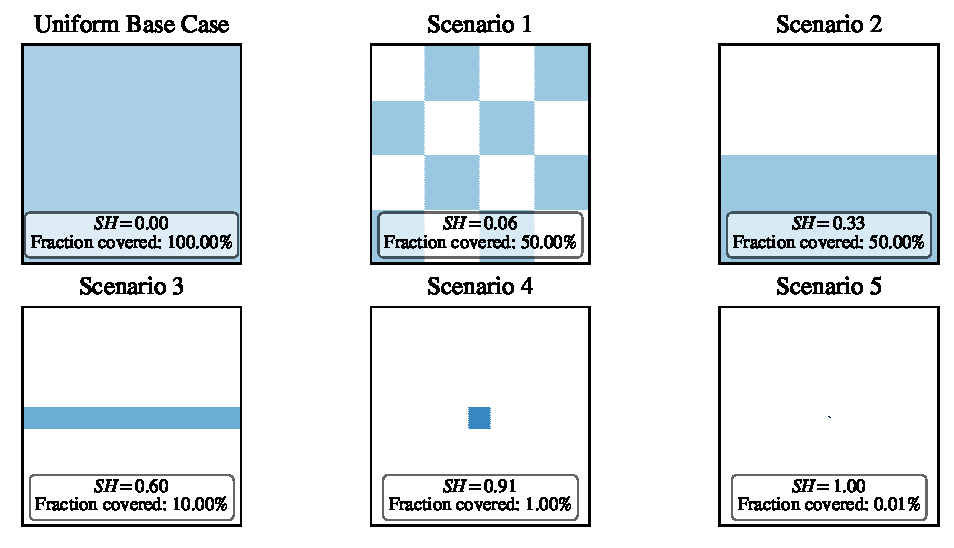
\includegraphics[width=\textwidth]{figures/chapter5/ideal-coag/ideal-coag-SH-scenarios.pdf}
    \caption{$SH$ scenarios for ideal coagulation simulations.}
    \label{fig:sh-scenarios-ideal-coag}
\end{figure}

Here we investigate the modification to the rate of coagulation under numerous spatial heterogeneity scenarios. We run a total of 6 simulations for a range of $SH$ scenarios shown in Figure \ref{fig:sh-scenarios-ideal-coag}. As with gas phase simulations in Chapter 4, the concentration of atmospheric constituents (here aerosol particle number concentration) must be scaled within the $SH$ scenario region by the ratio of the area of the uniform base case and the area occupied by the $SH$ pattern. For example, the aerosol number concentration in the central region of scenario 5 is a factor of 10,000 higher than in the uniform base case. 

Note that the setup of these simulations differs from all other simulations discussed in this thesis. Chemistry is turned off primarily for computational efficiency as, here, we are simply interested in changes to the number concentration rather than changes to aerosol composition. Instead of using initial conditions that are uniform throughout the domain, here the aerosol initial condition is set by the chosen $SH$ scenario for each vertical level in the domain (i.e., the pattern extends vertically throughout the domain). Additionally, emissions are turned off such that only coagulation is responsible for changes to aerosol number concentration.

\subsection{Results}

\begin{figure}[!h]
  \centering
    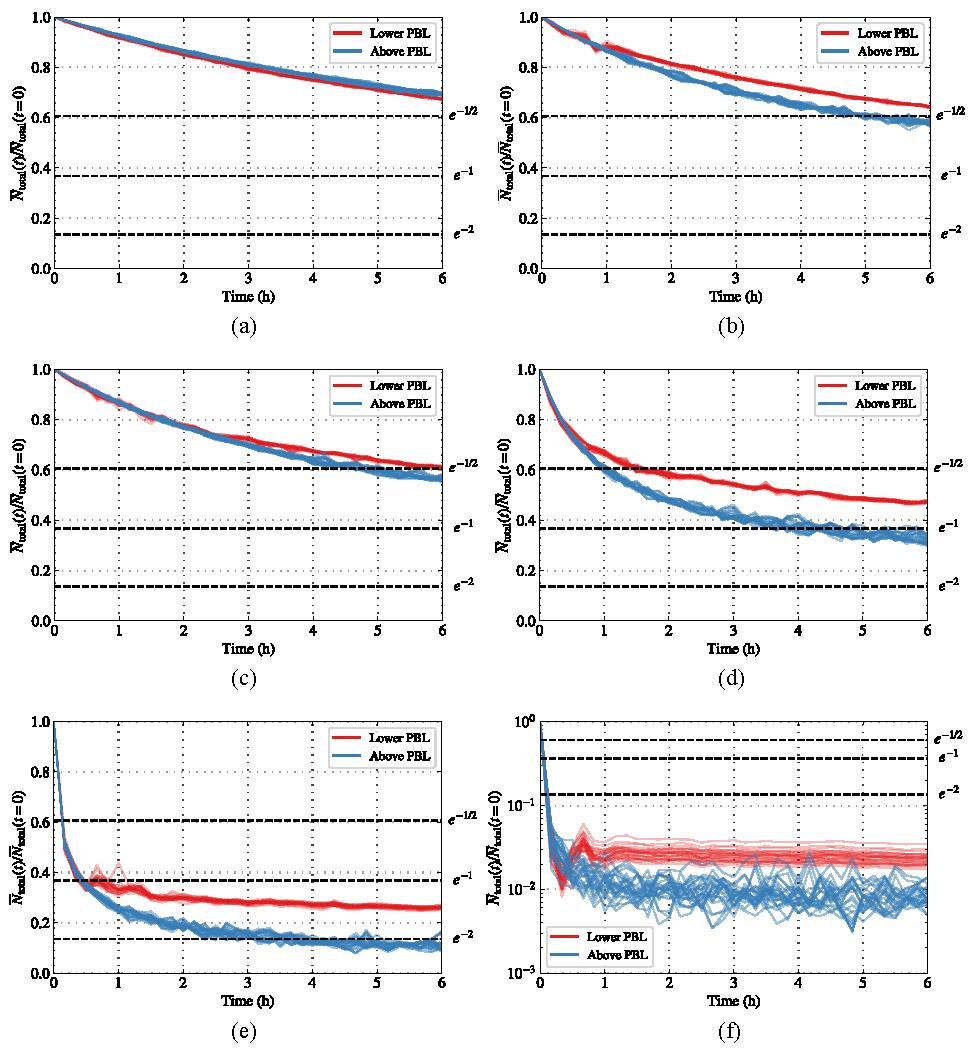
\includegraphics[width=\textwidth]{figures/chapter5/ideal-coag/NumConcTimescale_composite.pdf}
    \caption{Total number concentration for each $SH$ scenario normalized by the initial condition total number concentration. Lines indicate normalized number concentration averaged over each vertical level in the domain. (a) Uniform base case. (b--f) Scenarios 1--5}
    \label{fig:numconc-timescales}
\end{figure}

Figure \ref{fig:numconc-timescales} show how the total number concentration of aerosol particles decreases due to coagulation under each $SH$ scenario. For each scenario, we compute the average number concentration at each vertical level and time $t$, $\overline{N}_{\text{total}}(t)$. This number concentration is then normalized by the number concentration at time $t=0$, $\overline{N}_{\text{total}}(t=0)$. A subset of number concentration timeseries are shown in Figure \ref{fig:numconc-timescales} for the lowest 20 vertical levels of the PBL ($z=0$ m to $z\sim200$ m) and highest 20 vertical levels in the domain above the PBL ($z\sim1.8$ km to $z=2$ km). The reason for this grouping is that these two regions are notably different in terms of the rate at which the total number concentration decreases. For scenarios 1--5 (Figure \ref{fig:numconc-timescales} subfigures b--f), we find that the total number concentration decreases slower in the lower PBL than above the PBL. A notable exception to this trend is the uniform base case (Figure \ref{fig:numconc-timescales} subfigure a). Recall that the rate of coagulation scales as the square of the number of particles. As a result, highly heterogeneous patterns that require significant scaling up of the number concentration will have greater rates of coagulation within the high-concentration region associated with the $SH$ pattern. As the PBL develops and turbulent motion begins to diffuse the initial structure of the $SH$ pattern, concentration gradients are reduced, resulting in a reduction of the rate of coagulation. This turbulent motion does not disturb the structure of the $SH$ pattern above the PBL, and thus coagulation will proceed at a faster rate within the high concentration region of the $SH$ pattern.

We find that as the $SH$ increases across scenarios, the total number concentration is reduced more rapidly. For each plot in Figure \ref{fig:numconc-timescales}, we include horizontal dashed lines indicating the e-folding time alongside a half e-folding time ($e^{-1/2}$) and double e-folding time as the rate at which the total number concentration is reduced under $SH$ scenarios varies widely.  

\begin{figure}[t]
  \centering
    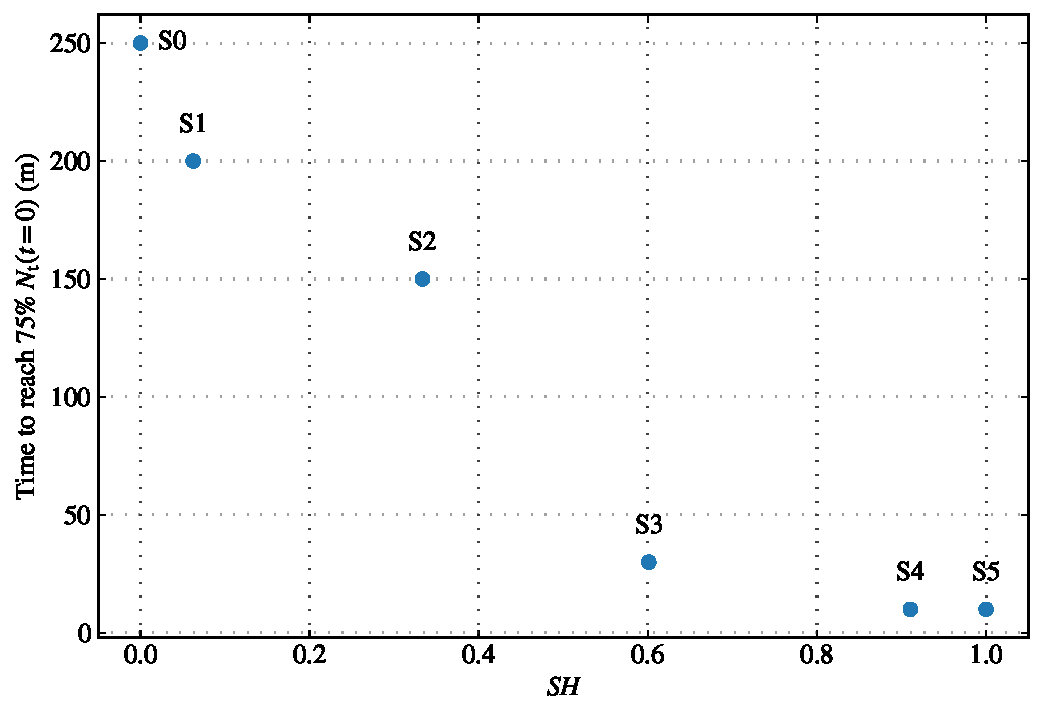
\includegraphics[width=\textwidth]{figures/chapter5/ideal-coag/TimeTo75pcnt_vs_SH.pdf}
    \caption{Time required in minutes for the total number concentration in the lowest 200 m of the PBL to be reduced to 75\% of the initial value vs. scenario $SH$. ``S0" is the uniform base case, with all other scenarios labeled S1--S5.}
    \label{fig:numconc-timescales-to-75pcent}
\end{figure}

Figure \ref{fig:numconc-timescales-to-75pcent} shows the time required the number concentration in the lower PBL to be reduced to 75\% of the initial total number concentration plotted against the spatial heterogeneity of each scenario. The uniform base case (``S0") requires over four hours to reach 75\% of the initial total concentration, while the highest heterogeneity scenarios 4 and 5 require only 10 minutes.

% --------------------------------------------
\section{Full multiphase simulations}

Here we discuss simulations containing full multiphase chemistry under numerous emissions spatial heterogeneity scenarios. A summary of emissions scenarios is presented followed by presentation of results pertaining to the aerosol state and properties under each emission scenario. 

\subsection{Simulated emissions scenarios}

\begin{figure}[t]
  \centering
    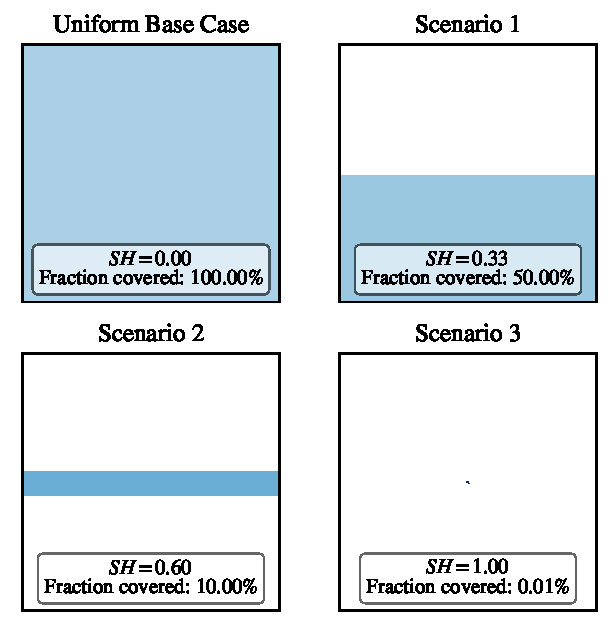
\includegraphics[width=.7\textwidth]{figures/SH-scenarios-main-runs.pdf}
    \caption{Emissions scenarios for multiphase chemistry simulations. The spatial heterogeneity of each emission scenario is listed in the lower portion of each scenario alongside domain mean and variance.
}
    \label{fig:aerosol-emission-scenarios}
\end{figure}

Scenarios discussed in this section match the set of emissions scenarios presented in Chapter 4 Section \ref{gas-emission-scenarios}. We evaluate changes to the aerosol population under four scenarios with increasing spatial heterogeneity as shown in Figure \ref{fig:aerosol-emission-scenarios}. As with previous results, the first scenario is a ``uniform base case", characterized by diffuse and uniform emissions across the ground level of the domain ($SH=0$). Scenarios 1--3 present progressively higher heterogeneity up to $SH=1$, whereby the rate of emissions is scaled to ensure the total mass per unit time emitted across each scenario is the same.

\subsection{Aerosol size distributions}

\begin{figure}[!t]
  \centering
    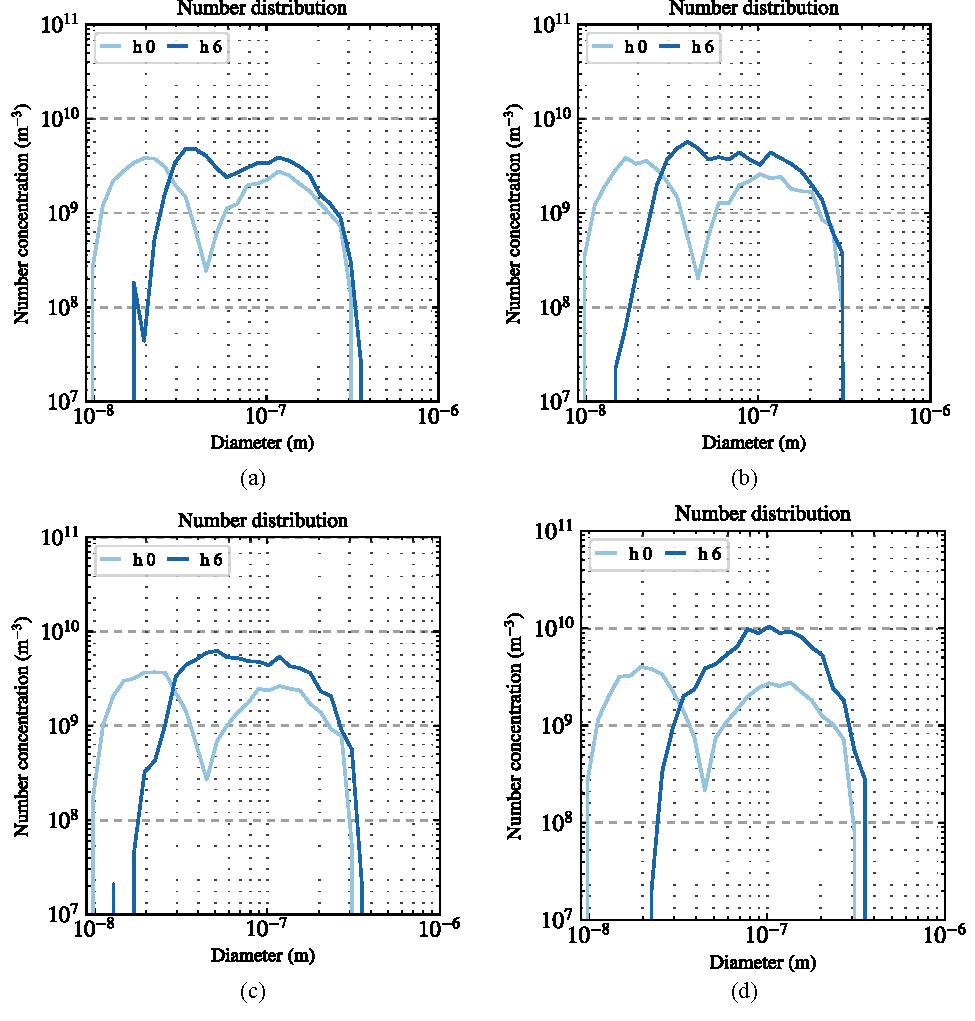
\includegraphics[width=\textwidth]{figures/chapter5/number-distribution-plots.pdf}
    \caption{Aerosol number distribution plots for each emissions scenario. The distribution initial condition (light blue) is shown alongside the distribution at the end of each simulation ($t=6$ h). Scenarios are labeled as the following: (a) uniform base case, (b) scenario 1, (c) scenario 2, (d) scenario 3.}
    \label{fig:number-dists}
\end{figure}

Figure \ref{fig:number-dists} shows aerosol number distributions for each simulated emissions scenario. The initial condition size distribution is presented alongside the size distribution at the end of each simulation ($t=6$ h). Each size distribution is taken from a vertical level in the upper boundary layer at $z\sim800$ \si{m}. Due to the stochastic treatment aerosols in the WRF-PartMC model and the chosen number of computational particles per grid cell ($n=100$), size distributions represent the average distribution in a 1 \si{km^2} region centered over the emissions plume. For all scenarios except scenario 1, this region is located at the center of the domain. For scenario 1, emissions are released in one half of the domain that is offset from the center, thus the averaging region for the size distribution is located in the center of the emissions plume. WRF-PartMC returns the number distribution in 100 logarithmically spaced bins ranging from $10^{-9}$ m to $10^{-3}$ m.

For each scenario displayed in Figure \ref{fig:number-dists}, the initial condition size distribution is shown in light blue. The distribution is bimodal, containing an Aitken (left) and accumulation mode (right). The Aitken mode contains fine particulates and is centered around $20$ nm, while the accumulation mode contains slightly fewer particles and is centered around 116 nm. 

After 6 hours, the number of particles with diameter smaller than $\sim30$ nm is significantly reduced as these small particles undergo coagulation and growth by gas-to-particle partitioning. For particle diameters greater than $\sim30$ nm, the number concentration is increased under each scenario as primary aerosol are emitted and particles undergo aging. For the uniform base case (Figure \ref{fig:number-dists} subplot a), the distribution still takes on a bimodal shape at $t=6$ h, however the Aitken mode has been replaced by a mode centered around 35 nm and is likely a combination of primary aerosol emissions and growth of smaller particles from the initial Aitken mode. 

Moving to higher emissions spatial heterogeneity scenarios, we find that the number distribution loses its bimodal shape after 6 hours, especially under the highest heterogeneity scenario, scenario 3 (Figure \ref{fig:number-dists} subplot d). For scenario 3, the number distribution peaks around 0.1 $\mu$m. Compared with the uniform base case, the number concentration of particles in the accumulation mode near $D_p = 0.1$ \si{\mu m} is approximately half an order of magnitude higher ($10^{10}$ \si{m^{-3}} vs. $4\cdot10^9$ \si{m^{-3}}).

\begin{figure}[!t]
  \centering
    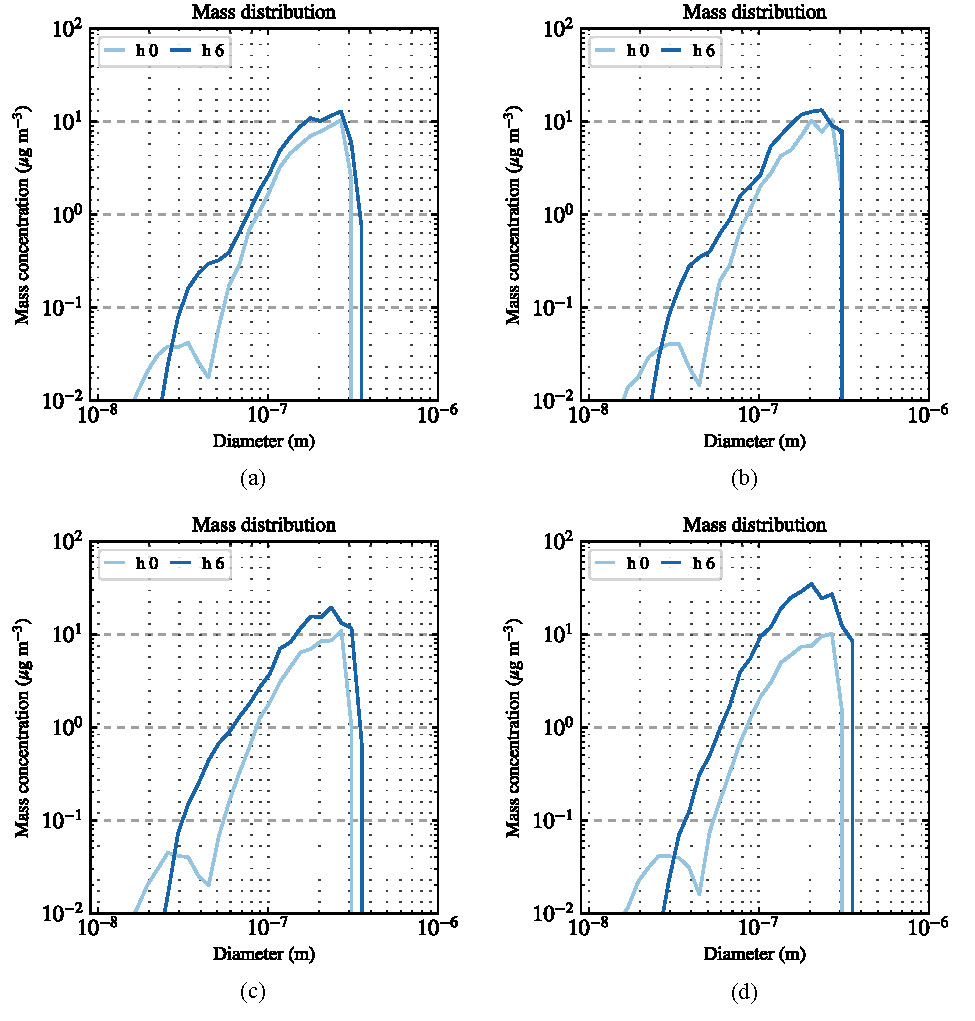
\includegraphics[width=\textwidth]{figures/chapter5/mass-distribution-plots.pdf}
    \caption{Aerosol mass distribution plots for each emissions scenario. The distribution initial condition (light blue) is shown alongside the distribution at the end of each simulation ($t=6$ h). Scenarios are labeled as the following: (a) uniform base case, (b) scenario 1, (c) scenario 2, (d) scenario 3.}
    \label{fig:mass-dists}
\end{figure}

Figure \ref{fig:mass-dists} shows mass distribution plots for each emissions scenario. Mass distributions were taken from the same upper boundary layer region as number distributions and the same averaging technique was applied over a 1 \si{km^2} region centered over the emissions plume. Mass concentrations are presented in \si{\mu g.m^{-3}}. 

The mass distribution initial condition presents a bimodal profile as before; however, much more mass is concentrated in the larger accumulation mode particles due to the cubic scaling between mass and particle diameter, $M_p \propto D_p^3$. After six hours, the mass concentration of all particles with diameters larger than $\sim25$ nm is increased. The distribution for the uniform base case (Figure \ref{fig:mass-dists} subfigure a) contains two distinct modes, one corresponding to the accumulation mode and an additional mode centered around $40--50$ nm. This mode likely contains primary aerosol emissions and particles that have grown from the Aitken mode due to aging processes. 

As with the number distributions, when moving from low to high $SH$ scenarios, the bimodal shape of the mass distribution is replaced by a single mode centered around the accumulation mode, peaking at $D_p = 0.2$ \si{\mu m}. When compared to the uniform base case, mass concentrations in the accumulation mode for the highest $SH$ case, scenario 3, are approximately 3 times higher ($\sim30$ \si{\mu g.m^{-3}} vs. $\sim10$ \si{\mu g.m^{-3}}).


\subsection{Aerosol composition}

\begin{figure}[!t]
  \centering
    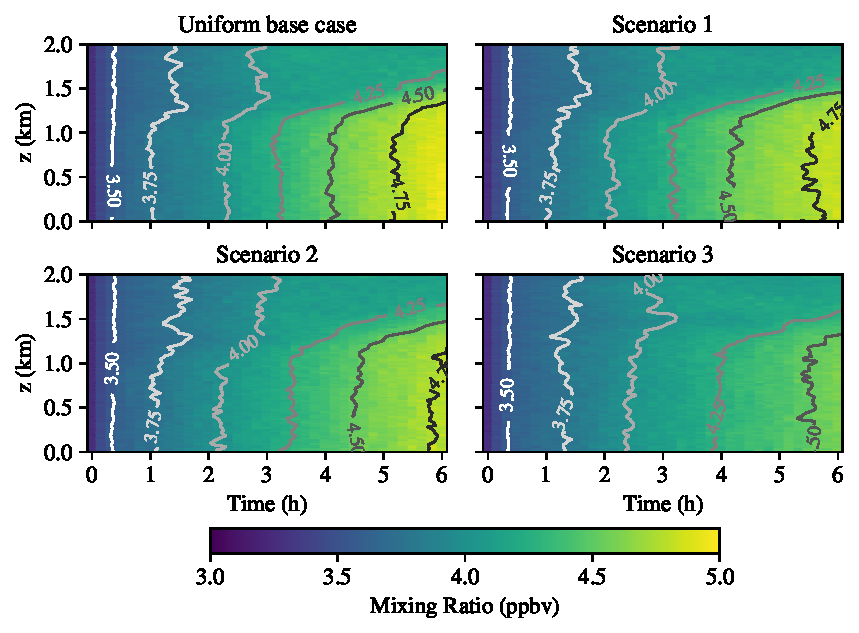
\includegraphics[width=\textwidth]{figures/chapter5/height-time-pmc_SO4-four-scenarios.pdf}
    \caption{Time-height plots for aerosol sulfate across each emissions scenario. Isopleths indicate sulfate mixing ratio in ppbv ranging from 3.5--4.75 ppbv.}
    \label{fig:ht-so4}
\end{figure}

Figure \ref{fig:ht-so4} shows time-height plots for aerosol sulfate concentrations in parts per billion by volume (ppbv). Mixing ratios are shown instead of mass concentrations as mixing ratio is independent of the atmospheric pressure and density. To compute the mixing ratio in ppbv for aerosol concentrations natively output by WRF-PartMC in \si{kg.m^{-3}}, concentrations are multiplied by the inverse of atmospheric density for each vertical level and by a factor of $10^9$ to convert from mol/mol to parts per billion.

As with previous time-height plots presented in Chapter 4, each pixel in the time-height grid mesh represents the average concentration over a given vertical level and time. Isopleths indicate lines of constant sulfate mixing ratios, ranging from 3.50 to 4.75 ppbv in increments of 0.25 ppbv.

Initially, each scenario contains a uniform sulfate concentration of $\sim3.5$ ppbv. During the first hour, concentrations gradually increase everywhere, likely due to the oxidation of ambient SO$_2$ and partitioning of resulting H$_2$SO$_4$ into the aerosol phase due to its extremely low volatility vapor pressure. As emissions turn on at $t=1$ h, the concentration of sulfate across emissions scenarios begins to diverge. In the uniform base case, sulfate concentrations steadily increase within the PBL through $t=6$ h up to 4.75 ppbv. For high $SH$ scenarios such as scenario 3, the rate of increase in sulfate concentrations is suppressed--it takes nearly two hours for sulfate concentrations to increase from 4.25 ppbv at $t=4$ h to 4.50 by $t=6$ h whereas the same increase under the uniform base case takes approximately 1 hour between $t=3$ h and $t=4$ h. This results in lower sulfate concentrations within the PBL under high $SH$ scenarios through $t=6$ h. For each scenario and timestep, we find that sulfate concentrations are approximately uniform throughout the PBL. 

\begin{figure}[!t]
  \centering
    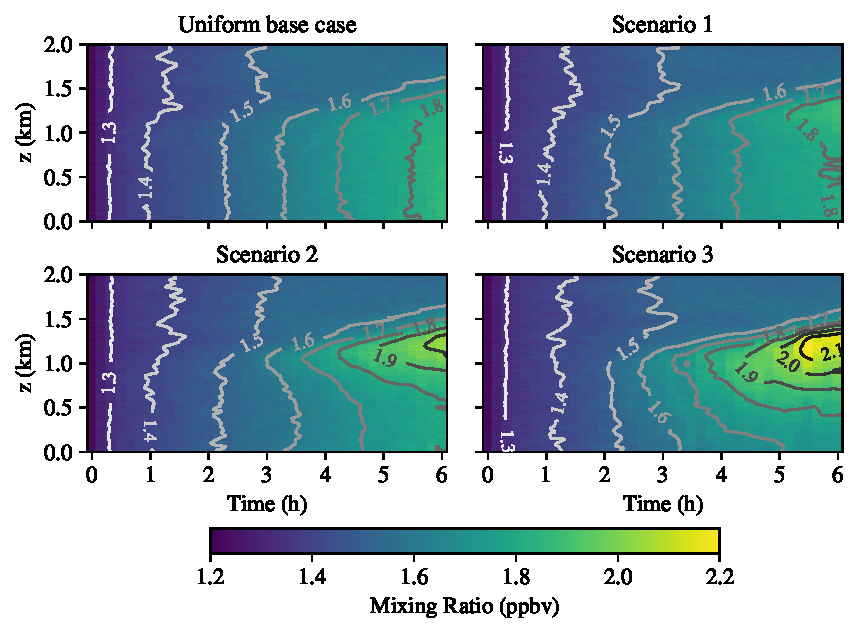
\includegraphics[width=\textwidth]{figures/chapter5/height-time-pmc_NH4-four-scenarios.pdf}
    \caption{Time-height plots for aerosol ammonium across each emissions scenario. Isopleths indicate ammonium mixing ratio in ppbv ranging from 1.3--2.1 ppbv.}
    \label{fig:ht-nh4}
\end{figure}

Time-height plots for ammonium concentrations in each emissions scenario are shown in Figure \ref{fig:ht-nh4}. Initially, aerosol ammonium concentrations are uniformly 1.2 ppbv everywhere. Ammonium concentrations steadily increase as ambient ammonia partitions into the aerosol phase. Following the release of emissions at $t=1$ h, ammonium concentrations are similar across each scenario between $t=1$ h to $t=2$ h with concentrations increasing to 1.5 ppbv. Subsequently, ammonium concentrations differ both spatially and temporally across emissions scenarios. Ammonium concentrations in the base case remain diffuse and relatively uniform throughout the PBL, increasing to 1.8 ppbv through $t=6$ h. As $SH$ increases across scenarios, ammonium concentrations in the upper PBL increase to as much as 2.1 ppbv in scenario 3 by $t=5$ to $t=6$ h. Meanwhile, concentrations in the lower PBL remain near 1.7--1.8 ppbv.

\begin{figure}[!t]
  \centering
    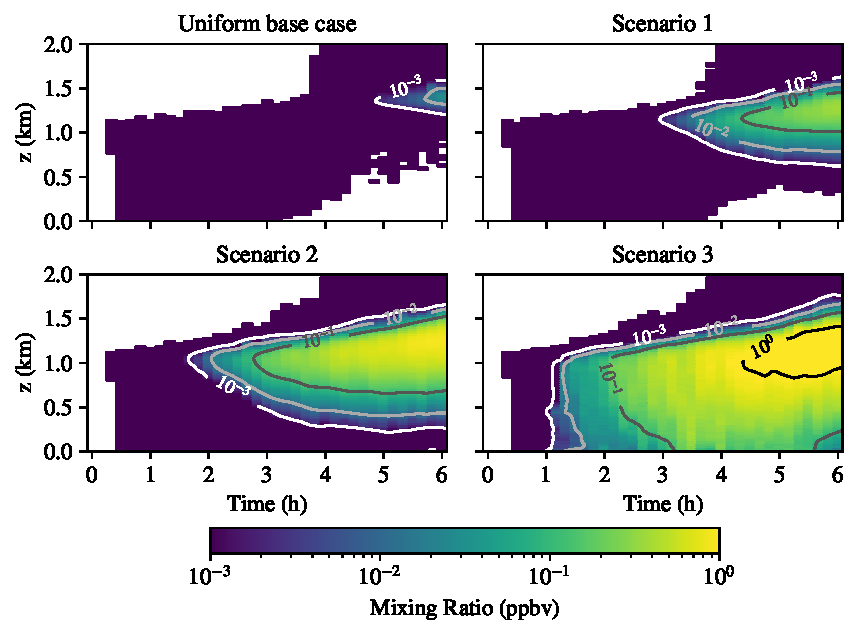
\includegraphics[width=\textwidth]{figures/chapter5/height-time-pmc_NO3-four-scenarios.pdf}
    \caption{Time-height plots for aerosol nitrate across each emissions scenario. Isopleths indicate nitrate mixing ratio in ppbv ranging from $10^{-3}$ to $10^0$ ppbv.}
    \label{fig:ht-no3}
\end{figure}

Figure \ref{fig:ht-no3} shows time-height plots of aerosol nitrate concentrations for each emissions scenario. Note the logarithmic scaling for the color bar as nitrate concentrations span numerous orders of magnitude due to trace concentrations in some regions. Initially, no nitrate is present in the aerosol phase (zero concentrations are indicated by white). Nitrate concentrations remain at or below $10^{-3}$ ppbv in the free troposphere throughout each scenario. When compared to sulfate and ammonium, the abundance of nitrate is most sensitive to emissions spatial heterogeneity as only trace amounts of nitrate ($10^{-3}$--$10^{-2}$ ppbv) are present in the upper PBL in the uniform base case, whereas concentrations reach 1 ppbv in the upper PBL in scenario 3. Additionally, the formation of nitrate occurs over a broader depth of the PBL for high $SH$ scenarios and the onset of formation occurs earlier. 

%\hl{Seinfeld and Pandis (10.4.4) discuss the SNA system and the two important regimes, ammonia-rich and ammonia-poor. In ammonia-poor, there isnt enough ammonia to neutralize the sulfate and most ammonia will exist in the gas phase and consequentially ammonium nitrate levels will also be low. In the ammonia rich case, there is excess ammonium than what is necessary to neutral all of the sulfate and thus the free ammonium will form ammonium nitrate.}

\begin{figure}[!t]
  \centering
    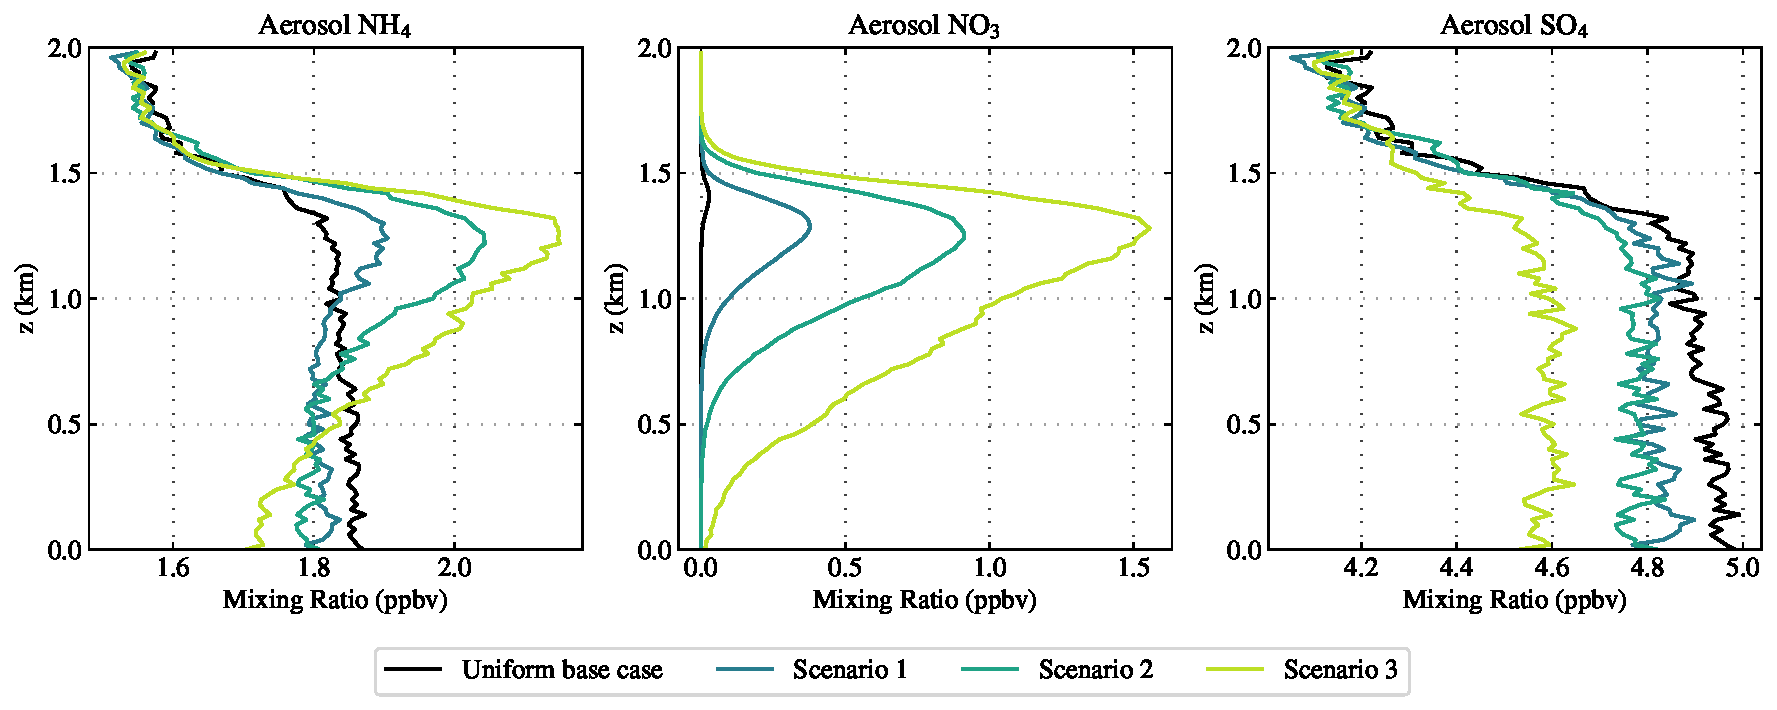
\includegraphics[width=\textwidth]{figures/chapter5/aerosol-SNA-vertical-profiles-time36.pdf}
    \caption{Vertical profiles of aerosol ammonia, nitrate, and sulfate at $t=6$ h.}
    \label{fig:sna-vertical-profile}
\end{figure}

Time-height plots for sulfate, ammonium, and nitrate capture the spatial and temporal variation of each aerosol species across each emissions scenario. However, to help quantitatively summarize and compare the relative abundances of each species, we focus here on the final state of the sulfate-nitrate-ammonium system at the end of each simulation, $t=6$ h. Figure \ref{fig:sna-vertical-profile} shows vertical profiles of ammonia, nitrate, and sulfate for $t=6$ h, whereby each vertical profile represents the horizontally averaged concentration in ppbv at each vertical level of the domain.

We find that ammonium has a relatively uniform concentration of 1.85 ppbv in the PBL for the uniform base case. As the spatial heterogeneity of emissions scenarios increases, the abundance of ammonium increases towards the upper PBL (which reaches a height of $z\sim1.5$ km by $t=6$ h), reaching 2.1 ppbv in the highest $SH$ scenario. Near the surface, ammonia concentrations decrease as the $SH$ of the emissions scenario increases. 

Nitrate levels increase with increasing emissions $SH$. For lower $SH$ scenarios, this increase is localized to the upper PBL. As emissions $SH$ increases across scenarios, nitrate concentrations also increase in the lower PBL, however the region of highest nitrate concentrations remains vertically distributed in the upper PBL. Nitrate levels reach up to 1.5 ppbv at $z\sim1.25$ km in the highest $SH$ scenario.  

Compared with ammonium and nitrate, sulfate concentrations within the PBL are more vertically uniform for each emissions scenario. As the $SH$ of emissions scenarios increases, sulfate concentrations are reduced by approximately the same amount everywhere in the PBL from a PBL average of 4.9 ppbv in the uniform base case to 4.6 ppbv in scenario 3. 

\begin{figure}[!t]
  \centering
    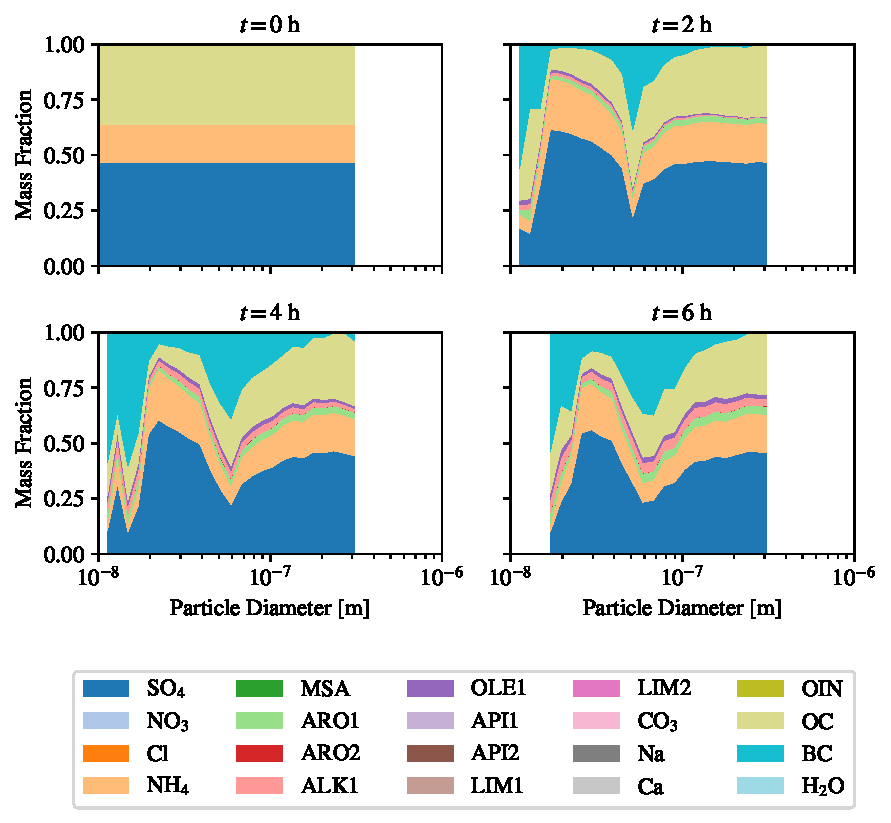
\includegraphics[width=\textwidth]{figures/chapter5/speciated-mass-frac-four-panel-uniform-basecase-z40.pdf}
    \caption{Size-resolved mass fraction for the uniform base case at regular 2-hour intervals.}
    \label{fig:mass-frac-ub}
\end{figure}

Figure \ref{fig:mass-frac-ub} shows the size-resolved mass fraction of aerosol particles in the upper PBL ($z\sim800$ m) at 2-hour intervals for the uniform base case. The average of species mass as a fraction of aerosol total mass is displayed for each aerosol species in WRF-PartMC. As with number and mass distribution plots, species concentrations are size-resolved with 100 logarithmically spaced bins between $10^{-9}$ and $10^{-3}$ m. Mass fractions are computed by dividing the mass of each species by the total mass of a bin. In order to reduce stochastic noise, an averaging strategy similar to that utilized for the number and mass distribution plots is employed, whereby mass fractions are computed for aerosol particles contained within a 1 \si{km^2} cross section of the domain centered over the emissions plume. Aerosol species model symbols are included in the key of Figure \ref{fig:mass-frac-ub}. A comprehensive list of aerosol species in WRF-PartMC is contained in Table \ref{table:wrf-partmc-species} alongside a description of each species model symbol". 

\begin{table}[!t]
\centering
\caption{Aerosol species and associated hygroscopicities in WRF-PartMC}
\begin{tabular*}{.6\linewidth}{@{\extracolsep{\fill}} lcc}
\\[-2ex]\hline 
     \hline \\[-2ex] \textbf{Aerosol species} & \textbf{Model symbol} & \textbf{Hygroscopicity $\kappa$} \\
\midrule
Sulfate & SO4 & 0.65 \\
Nitrate & NO3 & 0.65 \\
Chloride & Cl & 0.53 \\
Ammonium & NH4 & 0.65 \\
Nethanesulfonic acid & MSA & 0.53 \\
Aromatic & ARO1 & 0.1 \\
Aromatic & ARO2 & 0.1 \\
Alkanes & ALK1 & 0.1 \\
Olefin & OLE1 & 0.1 \\
$\alpha$-pinene & API1 & 0.1 \\
$\alpha$-pinene & API2 & 0.1 \\
Limonene & LIM1 & 0.1 \\
Limonene & LIM2 & 0.1 \\
Carbonate & CO3 & 0.53 \\
Sodium & Na & 0.53 \\
Calcium & Ca & 0.53 \\
Other inorganics & OIN & 0.1 \\
Organic carbon & OC & 0.001 \\
Black carbon & BC & 0 \\
Water & H2O & 0 \\
\\[-2ex]\hline 
     \hline \\[-2ex]
\end{tabular*}
\label{table:wrf-partmc-species}
\end{table}

For the initial condition, the composition of all particles is identical, with a mixture comprised of sulfate, organic carbon (OC), and ammonium. Once emissions are active at $t=1$ h, the release of carbonaceous primary aerosol introduces black carbon (BC) into the aerosol population.  By $t=6$ h, BC makes up a meaningful fraction of aerosol mass for fine particulates; particles with diameter $\sim20$ nm are up to 50\% BC and particles near 50--60 nm are $\sim40\%$ BC.

Additionally, volatile organic compounds (VOCs) are emitted in the gas phase which are oxidized, lowering their volatility and allowing them to condense into the aerosol phase as secondary organic aerosol (SOA). SOA species are organized by functional group in WRF-PartMC and include aromatics (``ARO1", ``ARO2"), alkanes (``ALK1", ``ALK2"), limonenes (``LIM1", ``LIM2"), etc (see Table \ref{table:wrf-partmc-species} for a full list). In size-resolved mass fraction plots, SOA appears as a ribbon of green, pink, and purple atop nitrate (orange), indicating that alkanes, olefins, and aromatics comprise the bulk of SOA species present in aerosol particles. In total, SOA makes up a small fraction of aerosol mass, reaching up to 10\% of total mass by $t=6$ h.

Throughout the uniform base case simulation, the mass fraction of sulfate makes up a large portion of aerosol mass. After initially being comprised of 45\% sulfate across all aerosol diameters, by $t=6$ h, sulfate mass fraction varies between a minimum of 10\% for ultrafine particles less than 20 nm and peaks at $\sim50\%$ for particles near 30 nm. Particles in the accumulation mode are comprised of 30--40\% sulfate. Ammonium initially comprises $\sim10\%$ of aerosol mass fraction and its relative contribution to total aerosol mass is fairly consistent across time, especially for larger particles ($D_p > 0.1$ \si{\mu m}). The mass fraction of ammonium reaches a minimum for particles ultrafine particles less than 30 nm in diameter. It is important to note that no nitrate is present at any point during the uniform base case simulation.

\begin{figure}[!t]
  \centering
    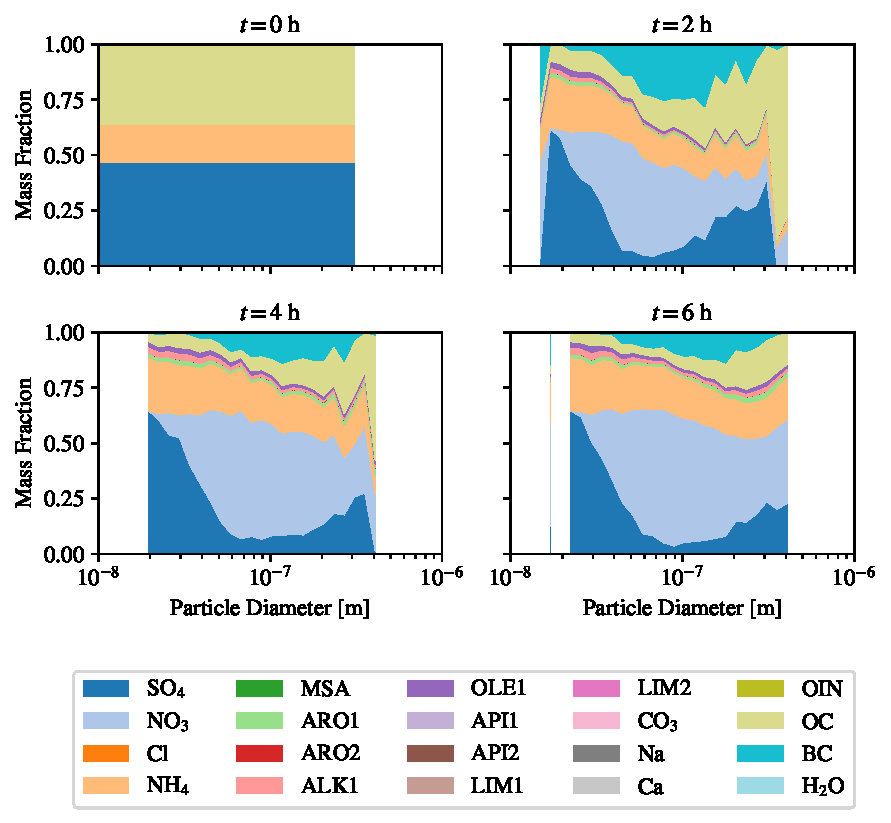
\includegraphics[width=\textwidth]{figures/chapter5/speciated-mass-frac-four-panel-point-source-1x1-z40.pdf}
    \caption{Size-resolved mass fraction for emissions scenario 3 at regular 2-hour intervals showing species mass fraction as a percent of total aerosol mass vs. particle diameter.}
    \label{fig:mass-frac-s3}
\end{figure}

Figure \ref{fig:mass-frac-s3} shows size-resolved mass fraction plots for the highest heterogeneity case, scenario 3. By $t=6$ h, the composition of aerosol particles is markedly different than in the uniform base case shown in Figure \ref{fig:mass-frac-ub}. Most notably, we find that nitrate comprises a large fraction of aerosol mass, especially for particle diameters near $D_p\sim0.1$ \si{\mu m}. As particle diameter decreases below 0.1 \si{\mu m}, the mass fraction of sulfate steady increases from less than 10\% to nearly 60\% for particles with diameter $D_p  \lesssim 30$ nm. Sulfate and nitrate effectively replace the large mass fraction of BC found for these ultrafine particles. By $t=6$ h, sulfate, nitrate, and ammonium jointly comprise a majority of aerosol mass across all particles diameters observed in emissions scenario 3. For particles smaller than 0.1 \si{\mu m}, sulfate, nitrate, and ammonium represent over 80\% of aerosol mass. For particles larger than 0.1 \si{\mu m}, these species comprise 70--80\% of aerosol mass.

Differences observed in aerosol composition are important due to the varying properties of aerosol species and their downstream influence on the atmospheric state. For example, particle hygroscopicity determines the critical supersaturation at which a particle of a given diameter will active as a cloud condensation nucleus. Hygroscopicity is parameterized using the $\kappa$-Köhler theory of \cite{petters_single_2007}. $\kappa$-Köhler theory is a modification to Köhler's relationship for determining the saturation ratio over a particle and the critical supersaturation at which the particle activates (\cite{kohler_nucleus_1936}). Each aerosol species has an associated hygroscopicity $\kappa$, and the total particle $\kappa$ is a volume-weighted sum of each species $\kappa$. Note that Table \ref{table:wrf-partmc-species} lists the hygroscopicity parameter $\kappa$ of each aerosol species and is highly variable (e.g., the hygroscopicity of BC is zero while sulfate has a hygroscopicity of 0.65). Values of  $\kappa$ greater than 0.5 indicate the aerosol species has a high hygroscopicity, while $\kappa=0$ corresponds to a nonhygroscopic compound.

\begin{figure}[!t]
  \centering
    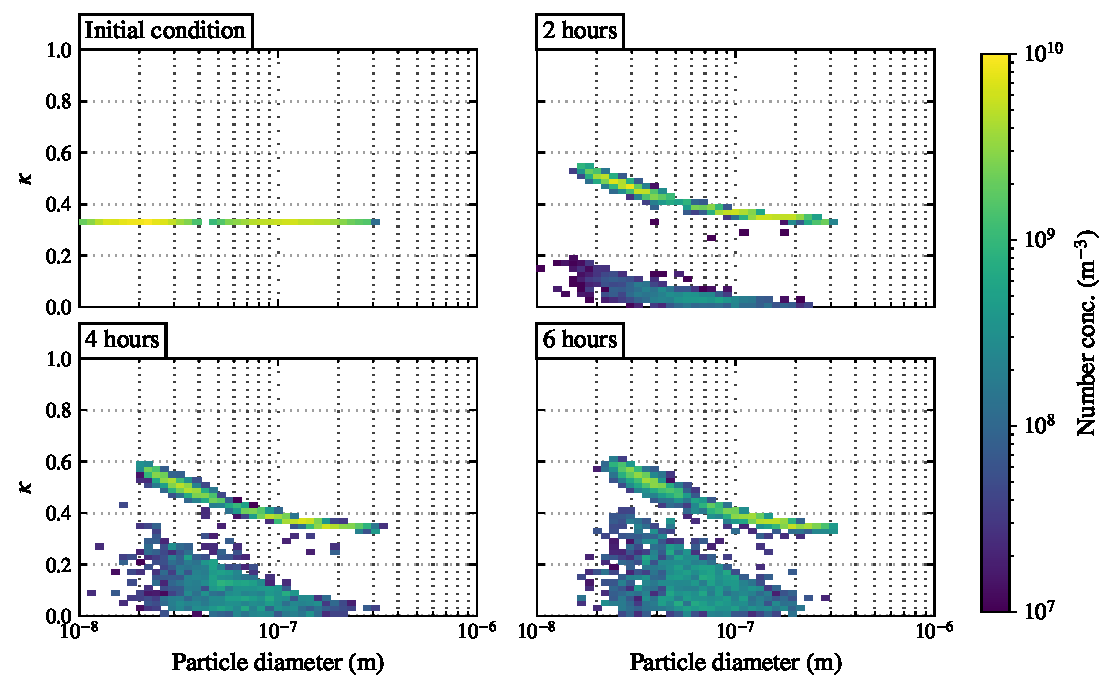
\includegraphics[width=\textwidth]{figures/chapter5/2d-kappa-dist-4-panel-uniform-basecase-z40.pdf}
    \caption{2-dimensional number distributions $n(D_p, \kappa)$ at regular two-hour intervals for the uniform base case.}
    \label{fig:2d-kappa-dist-ub}
\end{figure}

Figure \ref{fig:2d-kappa-dist-ub} shows two-dimensional number distributions at regular two hour intervals for the uniform base case in the upper PBL ($z\sim800$ m). The x-axis indicates particle diameter in meters, while hygroscopicity $\kappa$ is plotted along the y-axis. Particles are binned into a two-dimensional histogram by diameter (50 bins from 10 nm to 1 $\mu$m) and $\kappa$ (50 bins from 0 to 1) and the number concentration within each bin is tallied and displayed as a colorbar. Bins with zero particles are filled in white.

At the initial condition, we find that all particles posses the same total hygroscopicity, $\kappa=0.32$, as each is a mixture of ammonium sulfate and OC. Beginning at $t=1$ h, emissions of primary aerosol and gas phase species alter the distribution of particle hygroscopicity. Recall that emitted primary aerosol are composed of OC and BC with $\kappa$ values 0.001 and 0, respectively. This results in a distribution of low-$\kappa$ aerosol particles situated beneath the sulfate-rich aerosol. As the simulation evolves, gas-particle partitioning and coagulation age the aerosol population, increasing particle hygroscopicity.

\begin{figure}[!t]
  \centering
    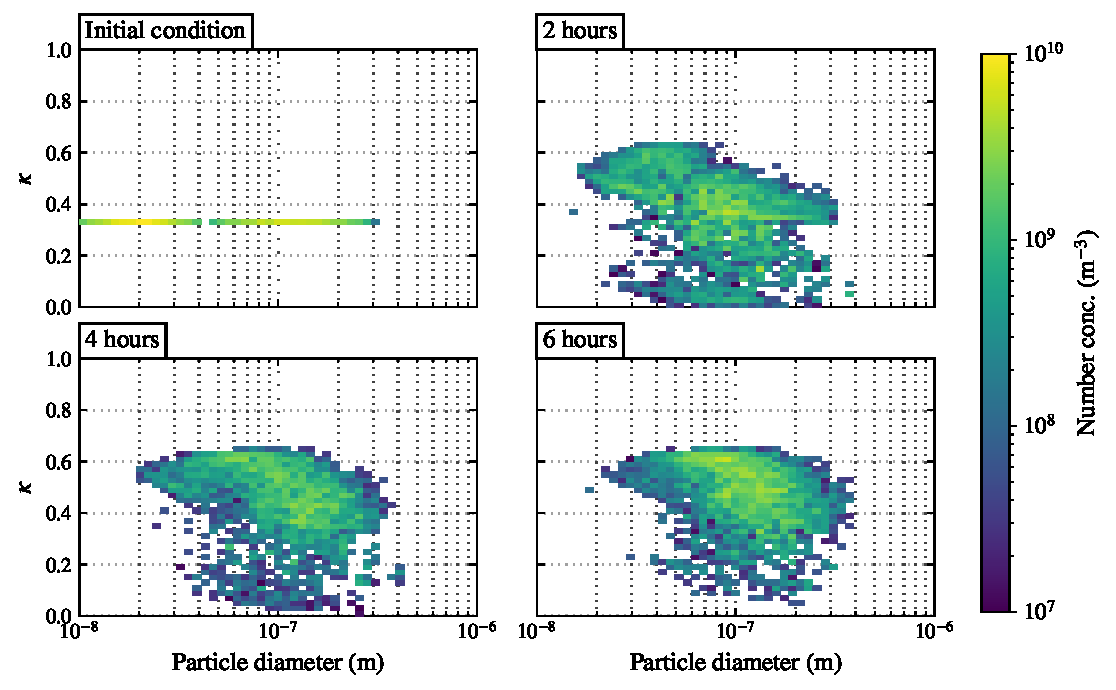
\includegraphics[width=\textwidth]{figures/chapter5/2d-kappa-dist-4-panel-point-source-1x1-z40.pdf}
    \caption{2-dimensional number distributions $n(D_p, \kappa)$ at regular two-hour intervals for scenario 3.}
    \label{fig:2d-kappa-dist-s3}
\end{figure}


\subsection{aerosol mixing state}

\begin{itemize}
\item Vertical profile of average particle $\chi$, $D_{\alpha}$, $D_{\gamma}$
\item Vertical profile of ccn $\chi$, $D_{\alpha}$, $D_{\gamma}$
\end{itemize}

\begin{figure}[!t]
  \centering
    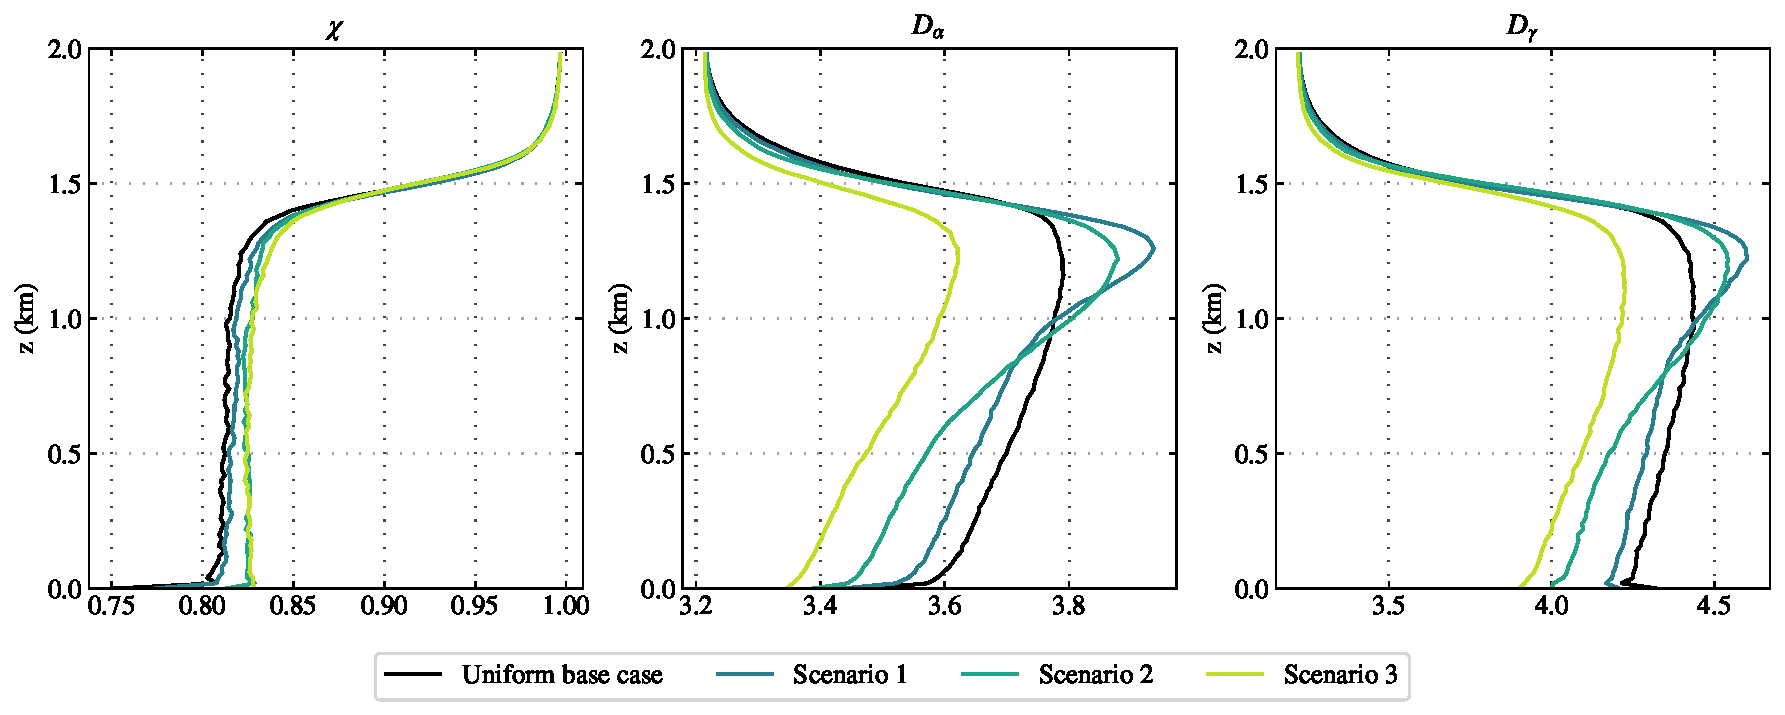
\includegraphics[width=\textwidth]{figures/chapter5/aerosol-mixingstate-vertical-profiles-time36.pdf}
    \caption{}
    %\label{fig:2d-kappa-dist-s3}
\end{figure}

\begin{figure}[!t]
  \centering
    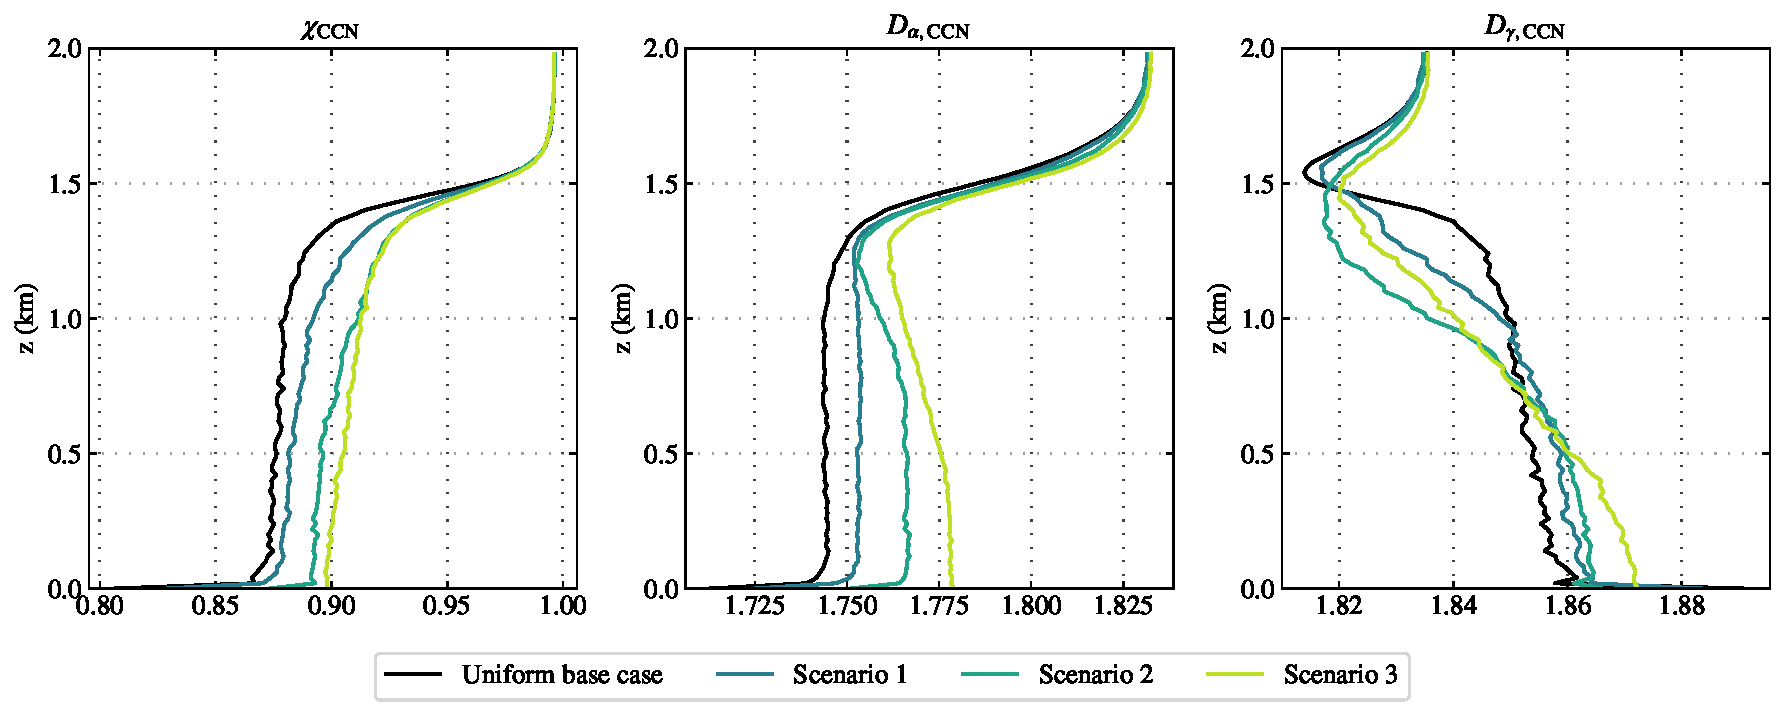
\includegraphics[width=\textwidth]{figures/chapter5/aerosol-ccn-mixingstate-vertical-profiles-time36.pdf}
    \caption{}
    %\label{fig:2d-kappa-dist-s3}
\end{figure}


\subsection{ccn}

\begin{itemize}
\item Vertical profile of ccn conc at each supersaturation level
\item Vertical profile of ccn $\chi$, $D_{\alpha}$, $D_{\gamma}$
\item time height plots of ccn \% error
\item (potentially) some sort of box plot ccn error thing similar to what I showed at IAMA?
\end{itemize}

\subsection{Runs without ammonia}

\begin{itemize}
\item Vertical profile of SNA
\item Vertical profile of ccn conc at each supersaturation level
\end{itemize}


\newpage
\begin{figure}[h]
  \centering
    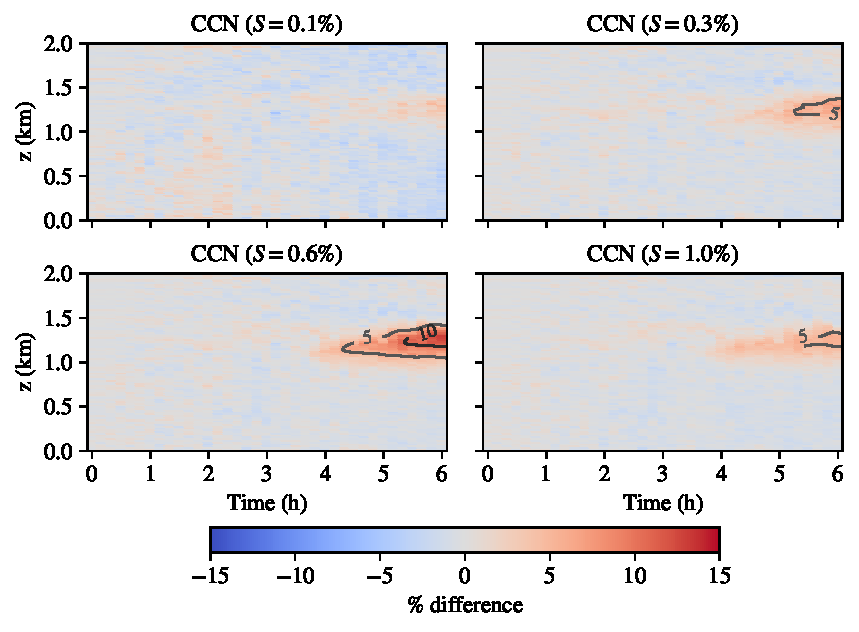
\includegraphics[width=\textwidth]{figures/chapter5/height-time-ccn-pdiff-fx1fy0.pdf}
    \caption{Scenario 1}
    \label{fig:ht-ccn-pdiff-s1}
\end{figure}

\newpage
\begin{figure}[h]
  \centering
    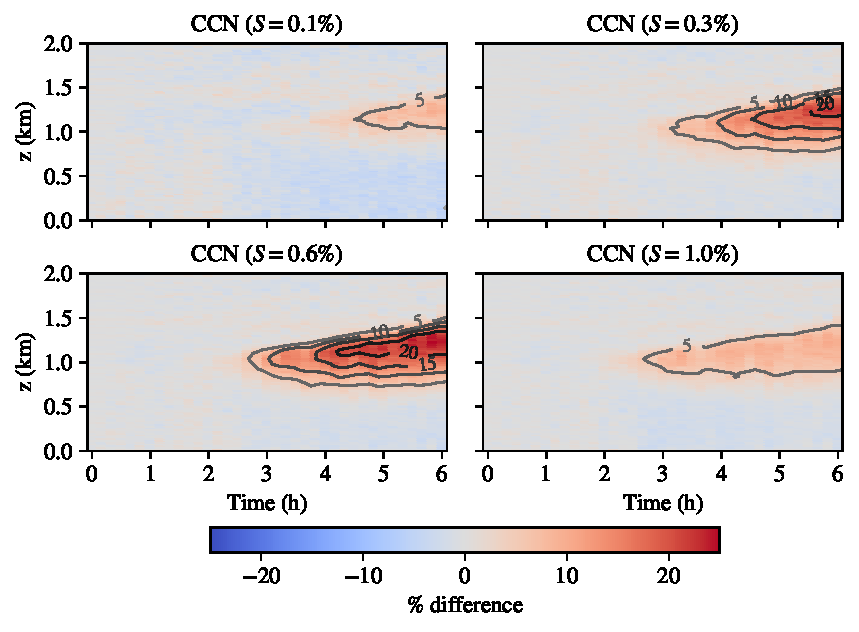
\includegraphics[width=\textwidth]{figures/chapter5/height-time-ccn-pdiff-road-10x.pdf}
    \caption{Scenario 2}
    \label{fig:ht-ccn-pdiff-s2}
\end{figure}

\newpage
\begin{figure}[h]
  \centering
    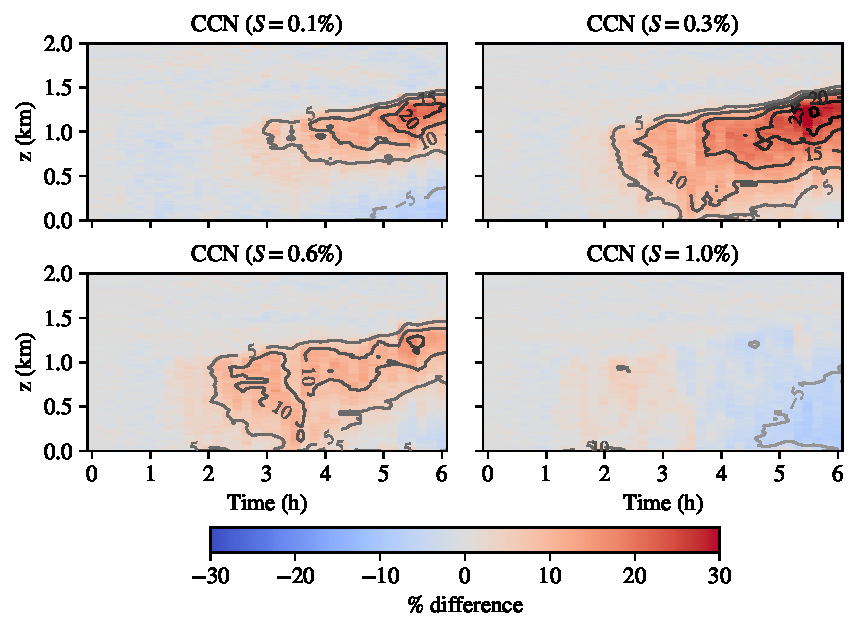
\includegraphics[width=\textwidth]{figures/chapter5/height-time-ccn-pdiff-point-source-1x1.pdf}
    \caption{Scenario 3}
    \label{fig:ht-ccn-pdiff-s3}
\end{figure}

